\documentclass{standalone}
\usepackage{tikz}
\usepackage{amsmath}
\usepackage{amssymb}
\usepackage{bm}

\newcommand{\ket}[1]{|#1\rangle}

\begin{document}

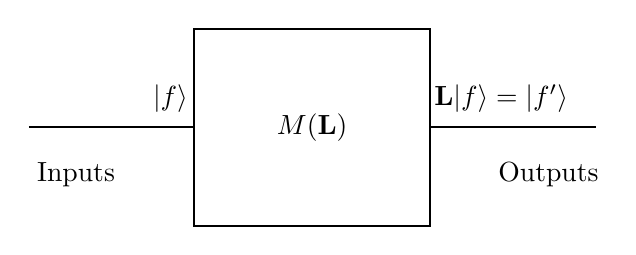
\begin{tikzpicture}[
  scale=1.2,
  thick,
  >=stealth,
  box/.style={draw, minimum width=3cm, minimum height=2.5cm}
]
  % Central box
  \node[box] (box) at (0,0) {$M(\mathbf{L})$};
  
  % Input wire
  \draw (-3,0) -- (box.west);
  \node at (-2.5,-0.5) {Inputs};
  \node at (-1.5,0.3) {$\ket{f}$};
  
  % Output wire
  \draw (box.east) -- (3,0);
  \node at (2.5,-0.5) {Outputs};
  \node at (2,0.3) {$\mathbf{L}\ket{f} = \ket{f'}$};
\end{tikzpicture}

\end{document}